\documentclass[aps,pre,preprint]{revtex4-1}
% \documentclass[aps,pre,twocolumn]{revtex4-1}
% \documentclass[aps,jcp,groupedaddress,twocolumn,unsortedaddress]{revtex4}

\usepackage{amsmath}
\usepackage{amssymb}
\usepackage[dvips]{graphicx}
\usepackage{color}
\usepackage{tabularx}

\makeatletter
\makeatother

\newcommand{\recheck}[1]{{\color{red} #1}}
\renewcommand{\v}[1]{\textbf{\textit{#1}}}
\renewcommand{\d}[1]{\textsf{#1}}
% \allowdisplaybreaks


\begin{document}

\title{The Error Estimate of Force Calculation in the Inhomogeneous Molecular Systems}
\author{Han Wang}
\affiliation{LMAM and School of Mathematical
  Sciences, Peking University}
\author{Pingwen Zhang}
% \email{pzhang@pku.edu.cn}
\affiliation{LMAM and School of Mathematical
  Sciences, Peking University}

\begin{abstract}
\end{abstract}

\maketitle

\section{Theory}
\subsection{Ewald summation}
The Ewald method divides the electrostatic interaction in to three
parts: the direct part, the reciprocal part and the correction
part. that is
\begin{equation}
E = E_{\textrm{dir}} + E_{\textrm{rec}} + E_{\textrm{corr}},
\end{equation}
where 
\begin {align}
E_{\textrm{dir}} & = \frac12 \sum^{\ast}_{\v n}
\sum_{i,j = 1}^{N} \frac{q_iq_j \textrm{erfc}(\beta \vert\v{r}_{ij} + \v{n}\vert)}
{\vert\v{r}_{ij} + \v{n}\vert} \\
E_{\textrm{rec}} & = \frac1{2\pi V} \sum_{\v m \neq 0}
\frac{\exp(-\pi^2\v m^2 / \beta^2)}{\v m^2} S(\v m) S(-\v m) \\
 E_{\textrm{corr}}& = -\frac\beta{\sqrt \pi} \sum_{i=1}^N q_i^2
\end {align}
The distance between the two particles is denoted by $\v r_{ij} = \v
r_i - \v r_j$, where $\v r_i$ and $\v r_j$ are positions of particle
$i$ and $j$, respectively.  The lattice in the real space is denoted
by $\v n = n_1 \v a_1 + n_2 \v a_2 + n_3 \v a_3$, where $\v a_\alpha,
\ \alpha=1,2,3$ are box vectors. the structure factor $S(\v m)$ is
defined by
\begin{equation}\label{sm1}
S(\v m) = \sum_{j=1}^N q_j \exp (2 \pi i \v m \cdot \v r_j),
\end{equation}
where $\v m = m_1 \v a_1^\ast + m_2 \v a_2^\ast + m_3 \v a_3^\ast$ is
the reciprocal space lattice vectors. $\v a_\alpha^\ast,\ \alpha = 1,
2, 3$ are conjugate reciprocal vectors of $\v a_\alpha$, defined by
$\v a_\alpha \cdot \v a_\beta^\ast = \delta_{\alpha\beta}$. and $V =
\v a_1 \cdot \v a_2 \times \v a_3$ is the volume of the box.

Both the direct and the reciprocal parts are calculated by cut-off in
real and reciprocal space, respectively. For the reciprocal part the
cut-offed energy reads
\begin{align}
  E_{\textrm{rec}} & =
  \frac1{2\pi V}
  \sum_{
    \begin{subarray}{c}
      \vert m_\alpha\vert < K_\alpha/2\\
      \v m\neq 0
    \end{subarray}}
  \frac{\exp(-\pi^2\v m^2 / \beta^2)}{\v m^2} S(\v m) S(-\v m)   
\end{align}
where $K_\alpha$ is the number of Fourier modes used on direction
$\alpha$. For convenience, we denote
\begin{align}
  f(\v m) = \frac{\exp(-\pi^2 \v m^2 / \beta^2)}{2\pi V \v m^2}
\end{align}
The truncated reciprocal force acting on particle $i$ is
\begin{align}
  \v F(\v r_i) = - 
  q_i 
  \sum_{
    \begin{subarray}{c}
      \vert m_\alpha\vert < K_\alpha/2\\
      \v m\neq 0
    \end{subarray}}
  \v g(\v m) \,
  S(-\v m)\,
  e^{2\pi i\v m\cdot\v r_i}
\end{align}
where
\begin{align}
  \v g(\v m) = -4 \pi \v m i f(\v m)
\end{align}



\subsection{Error estimate for the reciprocal Ewald force}

In this paper, we consider the force error, bacause the applicaions
are based on the molecular dynamics simulation.  Suppose the system is
composed by $N$ charged particles located at $\v r_1, \v r_2, \cdots,
\v r_N$ with charges $q_1, q_2, \cdots, q_N$, respectively.  We study
the force error of an arbitrary charge $i$ by the difference between
the exact force $\v F(\v r_i)$ and calculated force $\tilde{\v F}(\v
r_i)$ (with error introduced by cut-offs) exerting on the charge $i$.
The difference between the exact and calculated is called the
\emph{error force} \cite{short}, and is denoted by $\Delta \v F(\v r_i)
= \v F(\v r_i) - \tilde{\v F}(\v r_i)$.  The error of the force
computation is defined by the \emph{root mean square (RMS)}
\emph{error}, which is the square root of the second moment of the
error force: $\mathcal E(\v r_i) = \sqrt{\langle\vert\Delta\v F(\v
  r_i)\vert^2\rangle}$.  The notation $\langle\cdot\rangle$ means
ensemble average.

Ref.~\cite{wang2010optimizing} pointed out that it
is reasonable and convenient to estimate the error for the direct and
reciprocal force part seperately. 
The direct part is a short-range
interaction in real space, the error estimate of which
is well established in \cite{short}.
The mean of the error force is
\begin{align}\label{eqn:tmp10}
  \langle\Delta\v F_{\textrm{dir}}(\v r_i)\rangle
  =q_i\, [\v K^c_{\textrm{dir}}\ast\rho_q](\v r_i).
\end{align}
Herein, the ``$\ast$'' notation means convolution.  The direct
convolutional kernel of the error force $\v K^c_{\textrm{dir}}(\v r)$
is defined by
\begin{align}
  \v K^c_{\textrm{dir}}(\v r) =
  \left\{
    \begin{aligned}
      &\,0, &\quad & \vert\v r\vert \leq r_c;\\
      &,& & \vert\v r\vert > r_c,
      % \frac{\textrm{erfc}(\beta\vert\v r\vert)}{\vert\v r\vert}
    \end{aligned}
  \right.
\end{align}
where $r_c$ is the cut-off radius in the real space.  The first order
charge distribution function $\rho_q$ is defined by:
\begin{align}
  \rho_q(\v r) = 
  \bigg\langle
  \sum_{j = 1}^N
  \,q_j\,\delta(\v r - \v r_j)
  \bigg\rangle.
\end{align}
With the help of fast Fourier transform (FFT), the convolution in
\eqref{eqn:tmp10} can be calculated with the computational cost of
$\mathcal O(N\log N)$.

And the RMS error is estimated by
\begin{align}\nonumber
  \langle\vert\Delta\v F_{\textrm{dir}}(\v r_i)\vert^2\rangle
  = &\,
  q_i^2\,[(\v K^c_{\textrm{dir}})^2\ast\rho_{q^2}] (\v r_i) + 
  q_i^2\,[\v K^c_{\textrm{dir}}\ast\rho_{q}]^2 (\v r_i) + \\
  &
  q_i^2\,\int_{\mathbb R^3\times\mathbb R^3}
  \v K^c_{\textrm{dir}}(\v r_i-\v r')\cdot
  \v K^c_{\textrm{dir}}(\v r_i-\v r'')\,
  C_{q^2}(\v r', \v r'')\,
  \d d\v r'\d d\v r''.
\end{align}
The three terms on the right hand side are homogeneity error,
inhomogeneity error and correlation error. The inhomogeneity error is
nothing but the square of the mean error force \eqref{eqn:tmp10}. The
second order charge distribution $\rho_{q^2}$ is
\begin{align}
  \rho_{q^2}(\v r) = 
  \bigg\langle
  \sum_{j = 1}^N
  \,q^2_j\,\delta(\v r - \v r_j)
  \bigg\rangle.
\end{align}
The charge density correlation function is defined by
\begin{align}
  C_{q^2}(\v r', \v r'')
  =
  \bigg\langle
  \sum_{i\neq j}q_iq_j\delta(\v r'-\v r_i)\delta(\v r''-\v r_j)
  \bigg\rangle
  - \rho_q(\v r')\rho_q(\v r'').
\end{align}
In most situations, neglecting the correlation error will give
satisfactory estimate of the error~\cite{short}. Therefore, 
\begin{align}
  \langle\vert\Delta\v F_{\textrm{dir}}(\v r_i)\vert^2\rangle
  = &\,
  q_i^2\,[(\v K^c_{\textrm{dir}})^2\ast\rho_{q^2}] (\v r_i) + 
  q_i^2\,[\v K^c_{\textrm{dir}}\ast\rho_{q}]^2 (\v r_i).
\end{align}


The reciprocal error force, namely the difference between the
the exact and truncated reciprocal force, is
\begin{align}
  \Delta \v F_{\textrm{rec}}(\v r_i)
  = & - 
  q_i
  \sum_{\vert m_\alpha\vert \geq K_\alpha/2}
  \v g(\v m) \,
  S(-\v m)\,
  e^{2\pi i\v m\cdot\v r_i} 
\end{align}
It is proved that the mean reciprocal error force is
\begin{align}\label{eqn:tmp18}
  \big\langle
  \Delta \v F_{\textrm{rec}}(\v r_i)
  \big\rangle
  &= 
  -q_i\,[\v K^c_{\textrm{rec}}\ast\rho_q\,] (\v r_i),
\end{align}
where the reciprocal convolutional kernel of the error force $\v
K^c_{\textrm{rec}}$ is defined by:
\begin{align}
  \v K^c_{\textrm{rec}}(\v r) =
  \sum_{
      \vert m_\alpha\vert \geq K_\alpha/2}
  \v g(\v m) \,
  e^{2\pi i\v m\cdot\v r}.
\end{align}
Similarly, with the assumption of uncorrelation, it is shown that
\begin{align}
  \langle\vert\Delta\v F_{\textrm{rec}}(\v r_i)\vert^2\rangle
  = &\,
  q_i^2\,[(\v K^c_{\textrm{rec}})^2\ast\rho_{q^2}] (\v r_i) + 
  q_i^2\,[\v K^c_{\textrm{rec}}\ast\rho_{q}]^2 (\v r_i).
\end{align}


% Ref. \cite{short} pointed out that the inhomogeneity error is more
% harmful than the homogeneity error, so it is interesting to analyze
% the inhomogeneity error. Apply the Fourier transform on both sides of
% Eqn. \eqref{eqn:tmp10} and \eqref{eqn:tmp18}:
% \begin{align}  
%   \langle\Delta\v F_{\textrm{dir}}\rangle^\wedge(\v m)
%   &= q_i\,\hat{\v K}^c_{\textrm{dir}}(\v m)\cdot\hat\rho_q(\v m)\\
%   \langle\Delta\v F_{\textrm{rec}}\rangle^\wedge(\v m)
%   &= -q_i\,\hat{\v K}^c_{\textrm{rec}}(\v m)\cdot\hat\rho_q(\v m)
% \end{align}
% If the charge distribution is \emph{locally} neutral, then all modes
% of the first order density distribution vanishes, and $\langle\Delta\v
% F_{\textrm{dir}}\rangle = \langle\Delta\v F_{\textrm{rec}}\rangle = 0$.




\section{SPME}

The principle idea of the SPME method is to approximate the term
$e^{2\pi i\v m\cdot\v r}$ in the structure factor by the B-spline
interpolation. Denote the error introduced by this approximation by
$A(\v m, \v r)\,e^{2\pi i\v m\cdot \v r}$, we are fortunate to have
the analytical expression of $A(\v m, \v r)$:
\begin{align}
  A(\v m, \v r)
  =
  \sum_{\alpha=1}^3\sum_{l\neq 0}
  \frac
  {\big(\dfrac{2\pi m_\alpha}{K_\alpha} + 2\pi l\big)^{-n}}
  {\sum\limits_{l=-\infty}^{+\infty}
    \big(\dfrac{2\pi m_\alpha}{K_\alpha} + 2\pi l\big)^{-n}}
  \bigg(
  e^{2\pi i l K_\alpha\v a^\ast_\alpha\cdot \v r} - 1
  \bigg)
\end{align}

There are two possibility of calculating the reciprocal force from the
SPME energy. The first one is to differentiate the reciprocal term of
the original Ewald summation and then approximated the analytical
force by the B-spline interplation. This way is called
\emph{ik--differentiation}. The other way is to negative gradient on
the SPME approximated energy, as proposed in the original SPME paper
\cite{essmann1995spm}. The later is called \emph{analytical
differentiation}.


\subsection{Error estimate of the ik-differentiation}
The error force is 
\begin{align}\nonumber
  \Delta\v F^{\textrm{ik}}(\v r_i)
  =\;&
  q_i
  \sum_{
    \begin{subarray}{c}
      \vert m_{\alpha}\vert < K_\alpha/2\\
      \v m\neq 0
    \end{subarray}}
  \v g(\v m)\,
  A(\v m, \v r_i)\,
  e^{2\pi i\v m\cdot \v r_i}
  \sum_{j\neq i}q_j\,e^{-2\pi i\v m\cdot\v r_j} \\\nonumber
  & +\,
  q_i
  \sum_{
    \begin{subarray}{c}
      \vert m_{\alpha}\vert < K_\alpha/2\\
      \v m\neq 0
    \end{subarray}}
  \v g(\v m)\,
  e^{2\pi i\v m\cdot \v r_i}
  \sum_{j\neq i}q_j\,A(\v m, -\v r_j)\,e^{-2\pi i\v m\cdot\v r_j}\\\nonumber
  & +\,
  q_i
  \sum_{
    \begin{subarray}{c}
      \vert m_{\alpha}\vert < K_\alpha/2\\
      \v m\neq 0
    \end{subarray}}
  \v g(\v m)\,
  \big[
  A(\v m, \v r_i) +
  A(\v m, -\v r_i)
  \big]
\end{align}
The last ``self-interacting term'' is zero because of the symmetricity
of $\v g(\v m)$ and $A(\v m, \v r)$. 
By denoting
\begin{align}
  \v G_{\alpha,l}(\v r) =
  \sum_{
    \begin{subarray}{c}
      \vert m_{\alpha}\vert < K_\alpha/2\\
      \v m\neq 0
    \end{subarray}}
  \v g(\v m)\,
  \frac
  {\big(\dfrac{2\pi m_\alpha}{K_\alpha} + 2\pi l\big)^{-n}}
  {\sum\limits_{l=-\infty}^{+\infty}
    \big(\dfrac{2\pi m_\alpha}{K_\alpha} + 2\pi l\big)^{-n}}
  e^{2\pi i\v m\cdot\v r}
\end{align}
And if the high wave number terms are neglected, it is proved that the
mean error force is
\begin{align}
  \big\langle
  \Delta\v F^{\textrm{ik}}(\v r_i)
  \big\rangle
  & \approx
  - 2 q_i
  \bigg[
  \big(
  \sum_{\alpha}\sum_{l\neq 0}\v G_{\alpha,l}
  \big)
  \ast\rho_q\,
  \bigg] (\v r_i)
\end{align}
Also neglect the high wave number terms, the mean squared error force is 
\begin{align}\nonumber
  \big\langle
  \vert\Delta\v F^{\textrm{ik}}(\v r_i)\vert^2
  \big\rangle
  \approx&\, 
  2q_i^2
  \bigg[\,
  \big(
  \sum_{\alpha} \sum_{l\neq 0}
  \vert \v G_{\alpha,l}\vert^2
  \big)
  \ast \rho_{q^2}
  \,\bigg] (\v r_i)
  +
  4q_i^2\,
  \bigg[
  \big(
  \sum_{\alpha} \sum_{l\neq 0}  
  \v G_{\alpha,l}
  \big)^2
  \ast \rho_{q^2}\,
  \bigg] (\v r_i) \\
  &\,+
  \big\langle
  \Delta\v F^{\textrm{ik}}(\v r_i)
  \big\rangle  ^2
\end{align}






\subsection{Analytical differetiation}

The error force is 
\begin{align}\nonumber
  \Delta\v F^{\textrm{ana}}(\v r_i)
  =\;&
  q_i
  \sum_{
    \begin{subarray}{c}
      \vert m_{\alpha}\vert < K_\alpha/2\\
      \v m\neq 0
    \end{subarray}}
  -2f(\v m)\,
  \nabla_{\v r_i}
  e^{2\pi i\v m\cdot \v r_i}
  \sum_{j\neq i}q_j\,
  A(\v m, -\v r_j)
  e^{-2\pi i\v m\cdot\v r_j} \\\nonumber
  & +\,
  q_i
  \sum_{
    \begin{subarray}{c}
      \vert m_{\alpha}\vert < K_\alpha/2\\
      \v m\neq 0
    \end{subarray}}
  -2f(\v m)\,
  \nabla_{\v r_i}
  [A(\v m, \v r_i)\,
  e^{2\pi i\v m\cdot \v r_i} ]
  \sum_{j\neq i}q_j\,
  e^{-2\pi i\v m\cdot\v r_j} \\\nonumber
  & +\,
  q^2_i
  \sum_{
    \begin{subarray}{c}
      \vert m_{\alpha}\vert < K_\alpha/2\\
      \v m\neq 0
    \end{subarray}}
  -2f(\v m)\,
  A(-\v m, \v r_i)\,e^{2\pi i\v m\cdot \v r_i} \nabla_{\v r_i}e^{2\pi i\v m\cdot\v r_i} \\
  & +\,
  q^2_i
  \sum_{
    \begin{subarray}{c}
      \vert m_{\alpha}\vert < K_\alpha/2\\
      \v m\neq 0
    \end{subarray}}
  -2f(\v m)\,
  e^{-2\pi i\v m\cdot \v r_i}
  \nabla_{\v r_i} [\,A(\v m, \v r_i) \,e^{2\pi i\v m\cdot\v r_i}\,]  \\\nonumber
  =&\,
  \Delta\v F^{\textrm{ik}}(\v r_i)\\\nonumber
  & +\,
  q_i
  \sum_{
    \begin{subarray}{c}
      \vert m_{\alpha}\vert < K_\alpha/2\\
      \v m\neq 0
    \end{subarray}}
  -2f(\v m)\,
  \v B(\v m, \v r_i)\,e^{2\pi i\v m\cdot \v r_i}
  \sum_{j\neq i}q_j\,
  e^{-2\pi i\v m\cdot\v r_j} \\
  & +\,
  q^2_i
  \sum_{
    \begin{subarray}{c}
      \vert m_{\alpha}\vert < K_\alpha/2\\
      \v m\neq 0
    \end{subarray}}
  -2f(\v m)\,\v B(\v m, \v r_i) 
\end{align}
With $\v B(\v m, \v r)$ defined by
\begin{align}\nonumber
  \v B(\v m, \v r)
  &=
  \nabla_{\v r_i}A(\v m, \v r)\\
  &=
  \sum_{\alpha=1}^3\sum_{l\neq 0}
  \frac
  {\big(\dfrac{2\pi m_\alpha}{K_\alpha} + 2\pi l\big)^{-n}}
  {\sum\limits_{l=-\infty}^{+\infty}
    \big(\dfrac{2\pi m_\alpha}{K_\alpha} + 2\pi l\big)^{-n}}
  2\pi i l K_\alpha\v a_\alpha^\ast\,e^{2\pi i l K_\alpha\v a^\ast_\alpha\cdot \v r} 
\end{align}
For convenience, we denote
\begin{align}
  F_{\alpha,l} (\v r)
  &=
  \sum_{
    \begin{subarray}{c}
      \vert m_{\alpha}\vert < K_\alpha/2\\
      \v m\neq 0
    \end{subarray}}
  (-2)f(\v m)\,
  \frac
  {\big(\dfrac{2\pi m_\alpha}{K_\alpha} + 2\pi l\big)^{-n}}
  {\sum\limits_{l=-\infty}^{+\infty}
    \big(\dfrac{2\pi m_\alpha}{K_\alpha} + 2\pi l\big)^{-n}}\,
  e^{2\pi i\v m\cdot \v r}\\
  C_{\alpha,l}^{\textrm{self}}
  &= 
  \sum_{
    \begin{subarray}{c}
      \vert m_{\alpha}\vert < K_\alpha/2\\
      \v m\neq 0
    \end{subarray}}
  (-2)f(\v m)\,
  \frac
  {\big(\dfrac{2\pi m_\alpha}{K_\alpha} + 2\pi l\big)^{-n}}
  {\sum\limits_{l=-\infty}^{+\infty}
    \big(\dfrac{2\pi m_\alpha}{K_\alpha} + 2\pi l\big)^{-n}}\,
\end{align}
We prove:
\begin{align} \nonumber
  \langle \Delta\v F^{\textrm{ana}}(\v r_i)\rangle
  =\;&
  \langle \Delta\v F^{\textrm{ik}}(\v r_i)\rangle\\\nonumber
  &+\,
  q_i\sum_{\alpha}\sum_{l\neq 0}
  2\pi i\,l K_\alpha\v a_\alpha^\ast\,e^{2\pi i\,l K_\alpha\v a^\ast_\alpha\cdot \v r_i}
  [F_{\alpha,l}\ast\rho_q](\v r_i) \\\label{eqn:tmp30}
  &+\,
  q^2_i\sum_{\alpha}\sum_{l\neq 0}
  2\pi i\,l K_\alpha\v a_\alpha^\ast\,e^{2\pi i\,l K_\alpha\v a^\ast_\alpha\cdot \v r_i}
  C_{\alpha,l}^{\textrm{self}}
\end{align}
Neglecting all high frequency terms, we have:
\begin{align}\label{eqn:tmp31}
  \langle \Delta\v F^{\textrm{ana}}(\v r_i)\rangle
  \approx
  \langle \Delta\v F^{\textrm{ik}}(\v r_i)\rangle,
\end{align}
The ensemble average of the squared force error is
\begin{align}\nonumber
  \big\langle
  \vert \Delta\v F^{\textrm{ana}}(\v r_i)\vert^2
  \big\rangle
  =&\,
  q_i^2
  \bigg[\,
  \big(
  \sum_{\alpha} \sum_{l\neq 0}
  \vert \v G_{\alpha,l}\vert^2
  \big)
  \ast \rho_{q^2}
  \,\bigg] (\v r_i)\\\nonumber
  & +\,
  q_i^2
  \bigg[
  \big(
  \sum_{\alpha}\sum_{l\neq 0}
  \vert
  \v G_{\alpha,l} + 2\pi i\,l K_\alpha F_{\alpha,l} \v a_\alpha^\ast\vert^2
  \big)
  \ast \rho_{q^2}
  \bigg]
  (\v r_i) \\\nonumber
  & +\,
  4q_i^2\,
  \bigg[
  \big(
  \sum_{\alpha} \sum_{l\neq 0}  
  \v G_{\alpha,l}
  \big)^2
  \ast \rho_{q^2}\,
  \bigg] (\v r_i) \\
  & +\,
  \big\langle \Delta\v F^{\textrm{ana}}(\v r_i)\big\rangle ^2
\end{align}
It worthwhile noting that it will be problemetic to use
Eq. \eqref{eqn:tmp31} to calculate $\langle \Delta\v F^{\textrm{ana}}(\v r_i)\rangle
^2$, because by squaring the mean error force, the second and third
terms in Eq. \eqref{eqn:tmp30} will generate non-trivial low frequency
terms. Neglecting all high frequency terms, we have:
\begin{align}\nonumber
  \big\langle \Delta\v F^{\textrm{ana}}(\v r_i)\big\rangle ^2
  \approx&\,
  \big\langle \Delta\v F^{\textrm{ik}}(\v r_i)\big\rangle ^2 \\\nonumber
  &\,
  +q_i^2 \sum_{\alpha}\sum_{l\neq 0}
  4\pi^2l^2K_\alpha^2\vert\v a_{\alpha}^\ast\vert^2[F_{\alpha,l}\ast\rho_q]^2 (\v r_i) \\
  &\,
  +q_i^4 \sum_{\alpha}\sum_{l\neq 0}
  4\pi^2l^2K_\alpha^2\vert\v a_{\alpha}^\ast\vert^2[C_{\alpha,l}^{\textrm{self}}]^2 
\end{align}
the second one on the right hand side is always small, so
\begin{align}\nonumber
  \big\langle
  \vert \Delta\v F^{\textrm{ana}}(\v r_i)\vert^2
  \big\rangle
  =&\,
  q_i^2
  \bigg[\,
  \big(
  \sum_{\alpha} \sum_{l\neq 0}
  \vert \v G_{\alpha,l}\vert^2
  \big)
  \ast \rho_{q^2}
  \,\bigg] (\v r_i) \\\nonumber
  & +\,
  q_i^2
  \bigg[
  \big(
  \sum_{\alpha}\sum_{l\neq 0}
  \vert
  \v G_{\alpha,l} + 2\pi i\,l K_\alpha F_{\alpha,l} \v a_\alpha^\ast\vert^2
  \big)
  \ast \rho_{q^2}
  \bigg]
  (\v r_i) \\ \nonumber
  & +\,
  4q_i^2\,
  \bigg[
  \big(
  \sum_{\alpha} \sum_{l\neq 0}  
  \v G_{\alpha,l}
  \big)^2
  \ast \rho_{q^2}\,
  \bigg] (\v r_i) \\\nonumber
  & +\,
  \big\langle \Delta\v F^{\textrm{ik}}(\v r_i)\big\rangle ^2\\
  &+\,
  q_i^4 \sum_{\alpha}\sum_{l\neq 0}
  4\pi^2l^2K_\alpha^2\vert\v a_{\alpha}^\ast\vert^2[C_{\alpha,l}^{\textrm{self}}]^2 
\end{align}
the last one is a constant that stems from the self-interaction.



\section{Numerical tests}

We consider two inhomogeneous charge system to verify our error
estimate.  The first is locally neutral and globally inhomogeneous
charge system. In the second system, the positive and negative charges
are well seperated, while the number density of the charges is
uniform.

\subsection{Example 1: locally neutral}

In this example, 16800 charges are put into a $40\textsf{nm}\times
20\textsf{nm}\times 20\textsf{nm}$ periodic simulation box. Half of
them are carrying a unit positive charge of $+e$, and the other half
are carrying negative charge of $-e$. The position of these charges
are randomly generated subject to density distribution shown in
Fig.~\ref{fig:tmp-rho0}. Both the positive and negative charge
distributions are spacially inhomogeneous, while the system is locally
neutral, because the positive and negative charge distributions cancel
each other.

\begin{figure}
  \centering
  \includegraphics[width=.48\textwidth]{fig/error.one_peak.box40x20x20.b1.000.r3.00.n6.K101x051x051/fig.rho.eps}
  \caption{Charge distribution of Example 1. The red line
    denotes the positive charge distribution, while the blue line
    denotes the negative charge distribution. Since all distributions
    are uniform on $y$ and $z$ direction, they are plotted as a
    function of $x$.}
  \label{fig:tmp-rho0}
\end{figure}

\begin{figure}
  \centering
  \includegraphics[]{fig/error.one_peak.box40x20x20.b1.000.r3.00.n6.K101x051x051/fig.ana.ewald.meanf.eps}
  \caption{Example 1: the actual (denoted by dots) and estimated
    (denoted by straight lines) mean error force of the direct part
    $\langle\Delta \v F_{\textrm{dir}}(\v r)\rangle$ (red), reciprocal
    part of Ewald summation $\langle\Delta \v F_{\textrm{rec}}(\v
    r)\rangle$ (green) and the reciprocal part of the analytical
    differentiation $\langle\Delta \v
    F^{\textrm{ana}}_{\textrm{rec}}(\v r)\rangle$ (blue). The total
    mean error force of analytical differentiation $\langle\Delta \v
    F^{\textrm{ana}}(\v r)\rangle$ is given in pink.  Since the charge
    distribution is uniform on the $y$ and $z$ direction, the $y$ and
    $z$ dimension of the mean error force is averaged, and the errors
    are plotted on $x$ direction.  The cut-off in the real space is 3
    \textsf{nm}, the number of freedom in the reciprocal space is
    $100\times 50\times 50$, the parameter $\beta$ is $1.0\;
    \textsf{nm}^{-1}$ and the order of B-spline interpolation used for
    the analytical differentiation is 6.}
  \label{fig:meanf1}
\end{figure}

\begin{figure}
  \centering
  \includegraphics[]{fig/error.one_peak.box40x20x20.b1.000.r3.00.n6.K101x051x051/fig.ana.ewald.error.eps}
  \caption{Example 1: the actual (denoted by dots) and estimated
    (denoted by straight lines) RMS force error of the direct part
    $\sqrt{\langle\vert\Delta \v F_{\textrm{dir}}(\v
      r)\vert^2\rangle}$ (red), reciprocal part of Ewald summation
    $\sqrt{\langle\vert\Delta \v F_{\textrm{rec}}(\v
      r)\vert^2\rangle}$ (green) and the reciprocal part of the
    analytical differentiation $\sqrt{\langle\vert\Delta \v
      F^{\textrm{ana}}_{\textrm{rec}}(\v r)\vert^2\rangle}$
    (blue). The RMS force error of analytical differentiation
    $\sqrt{\langle\vert\Delta \v F^{\textrm{ana}}(\v
      r)\vert^2\rangle}$ is given in pink.  Since the charge
    distribution is uniform on the $y$ and $z$ direction, the $y$ and
    $z$ dimension of the mean error force is averaged, and the errors
    are plotted on $x$ direction.  The cut-off in the real space is 3
    \textsf{nm}, the number of freedom in the reciprocal space is
    $100\times 50\times 50$, the parameter $\beta$ is $1.0\;
    \textsf{nm}^{-1}$ and the order of B-spline interpolation used for
    the analytical differentiation is 6.}
  \label{fig:error1}
\end{figure}

% \begin{figure}
%   \centering
%   \includegraphics[width=.48\textwidth]{fig/error.one_peak.box40x20x20.b1.000.r3.00.n6.K101x051x051/fig.ik.meanf.eps}
%   \includegraphics[width=.48\textwidth]{fig/error.one_peak.box40x20x20.b1.000.r3.00.n6.K101x051x051/fig.ana.meanf.eps}
%   \caption{Resulting mean error force}
%   \label{fig:tmp1}
% \end{figure}

% \begin{figure}
%   \centering
%   \includegraphics[width=.48\textwidth]{fig/error.one_peak.box40x20x20.b1.000.r3.00.n6.K101x051x051/fig.ik.error.eps}
%   \includegraphics[width=.48\textwidth]{fig/error.one_peak.box40x20x20.b1.000.r3.00.n6.K101x051x051/fig.ana.error.eps}
%   \caption{Resulting RMS errors}
%   \label{fig:tmp2}
% \end{figure}

\subsection{Example 2: seperated positive and negative charge}

\begin{figure}
  \centering
  \includegraphics[width=.48\textwidth]{fig/error.two_peaks_sep.box40x20x20.b1.000.r3.00.n6.K101x051x051/fig.rho.eps}
  \caption{Charge distribution of Example 2. The red line
    denotes the positive charge distribution, while the blue line
    denotes the negative charge distribution. Since all distributions
    are uniform on $y$ and $z$ direction, they are plotted as a
    function of $x$.}
  \label{fig:tmp-rho2}
\end{figure}

\begin{figure}
  \centering
  \includegraphics[]{fig/error.two_peaks_sep.box40x20x20.b1.000.r3.00.n6.K101x051x051/fig.ana.ewald.meanf.eps}
  \caption{Example 2: the actual (denoted by dots) and estimated
    (denoted by straight lines) mean error force of the direct part
    $\langle\Delta \v F_{\textrm{dir}}(\v r)\rangle$ (red), reciprocal
    part of Ewald summation $\langle\Delta \v F_{\textrm{rec}}(\v
    r)\rangle$ (green) and the reciprocal part of the analytical
    differentiation $\langle\Delta \v
    F^{\textrm{ana}}_{\textrm{rec}}(\v r)\rangle$ (blue). The total
    mean error force of analytical differentiation $\langle\Delta \v
    F^{\textrm{ana}}(\v r)\rangle$ is given in pink.  Since the charge
    distribution is uniform on the $y$ and $z$ direction, the $y$ and
    $z$ dimension of the mean error force is averaged, and the errors
    are plotted on $x$ direction.  The cut-off in the real space is 3
    \textsf{nm}, the number of freedom in the reciprocal space is
    $100\times 50\times 50$, the parameter $\beta$ is $1.0\;
    \textsf{nm}^{-1}$ and the order of B-spline interpolation used for
    the analytical differentiation is 6.}
  \label{fig:meanf2}
\end{figure}


\begin{figure}
  \centering
  \includegraphics[]{fig/error.two_peaks_sep.box40x20x20.b1.000.r3.00.n6.K101x051x051/fig.ana.ewald.error.eps}
  \caption{Example 2: the actual (denoted by dots) and estimated
    (denoted by straight lines) RMS force error of the direct part
    $\sqrt{\langle\vert\Delta \v F_{\textrm{dir}}(\v
      r)\vert^2\rangle}$ (red), reciprocal part of Ewald summation
    $\sqrt{\langle\vert\Delta \v F_{\textrm{rec}}(\v
      r)\vert^2\rangle}$ (green) and the reciprocal part of the
    analytical differentiation $\sqrt{\langle\vert\Delta \v
      F^{\textrm{ana}}_{\textrm{rec}}(\v r)\vert^2\rangle}$
    (blue). The RMS force error of analytical differentiation
    $\sqrt{\langle\vert\Delta \v F^{\textrm{ana}}(\v
      r)\vert^2\rangle}$ is given in pink.  Since the charge
    distribution is uniform on the $y$ and $z$ direction, the $y$ and
    $z$ dimension of the mean error force is averaged, and the errors
    are plotted on $x$ direction.  The cut-off in the real space is 3
    \textsf{nm}, the number of freedom in the reciprocal space is
    $100\times 50\times 50$, the parameter $\beta$ is $1.0\;
    \textsf{nm}^{-1}$ and the order of B-spline interpolation used for
    the analytical differentiation is 6.}
  \label{fig:error2}
\end{figure}


% \begin{figure}
%   \centering
%   \includegraphics[width=.48\textwidth]{fig/error.two_peaks_sep.box40x20x20.b1.000.r3.00.n6.K101x051x051/fig.ik.meanf.eps}
%   \includegraphics[width=.48\textwidth]{fig/error.two_peaks_sep.box40x20x20.b1.000.r3.00.n6.K101x051x051/fig.ana.meanf.eps}
%   \caption{Resulting mean error force}
%   \label{fig:tmp3}
% \end{figure}

% \begin{figure}
%   \centering
%   \includegraphics[width=.48\textwidth]{fig/error.two_peaks_sep.box40x20x20.b1.000.r3.00.n6.K101x051x051/fig.ik.error.eps}
%   \includegraphics[width=.48\textwidth]{fig/error.two_peaks_sep.box40x20x20.b1.000.r3.00.n6.K101x051x051/fig.ana.error.eps}
%   \caption{Resulting RMS errors}
%   \label{fig:tmp4}
% \end{figure}





\newpage
\appendix
\section{Error estimate of the Ewald summation}




\newpage

\bibliography{ref}{}
\bibliographystyle{unsrt}


\end{document}
